% Preamble
\documentclass[10pt]{ltjsarticle}

% Packages
\usepackage{amsmath}
\usepackage{mathtools}
% \usepackage[backend=biber,sorting=none]{biblatex}
\usepackage{graphicx}
\usepackage{booktabs}
\usepackage{siunitx}
\usepackage{bm}
\usepackage{physics}

\mathtoolsset{showonlyrefs} % 参照した式のみ番号を表示
% \addbibresource{.bib}
% title
\title{東京大学院試物理学第3問}
\date{}

\begin{document}
    \maketitle
    下記の問題で、
    \begin{align}
        \vb{E} = E_r \vb{e}_r
    \end{align}
    であり、マクスウェル方程式から
    \begin{equation}
        \nabla^2 \vb{E} = \mu\epsilon \pdv[2]{\vb{E}}{t}
    \end{equation}
    なので
    \begin{equation}\label{eq:wave}
        \nabla^2 E_r = \mu\epsilon \pdv[2]{E_r}{t}.
    \end{equation}
    一方、小問3の形に電場を置くと
    \begin{equation}
        \div{\vb{E}} = \frac{1}{r}\dv{r} \qty(r \mathcal{E})e^{i(kz - \omega t)} = 0
    \end{equation}
    から
    \begin{equation}
        E_r = \frac{C}{r}, \hspace*{2em} C = const.\\
    \end{equation}
    $E_r(r = a) = \frac{C}{a} = E_0 $より $C = aE_0$.よって
    \begin{equation}
        E_r = \frac{E_0 a}{r}.
    \end{equation}
    しかしこれを波動方程式~\eqref{eq:wave}に代入すると
    \begin{align}
        \nabla^2 E_r - \mu\epsilon \pdv[2]{E_r}{t} 
        &= \qty{\frac{1}{r}\pdv{r}\qty(r \pdv{r}\qty(\frac{E_0 a}{r})) + (- k^2 + \mu \epsilon \omega^2) \frac{E_0 a}{r}}e^{i(kz - \omega t)}\label{eq:r} \\
        &= \frac{E_0 a}{r} \qty{\frac{1}{r^2} + (- k^2 + \mu \epsilon \omega^2)}e^{i(kz - \omega t)} \\
        &= 0
    \end{align}
    となり、正しくない。

    ここでわからなくなってしまったのですが、これは波動方程式が間違っているためなのか、$E_r$の形が間違っているためなのか、どちらなのでしょうか。
    もしくは計算間違えでしょうか。\eqref{eq:r}の第1項
    \begin{equation}
        \frac{1}{r}\pdv{r}\qty(r \pdv{r}\qty(\frac{E_0 a}{r}))
    \end{equation}
    が消えてくれないと、z軸方向に進む波の式としてふさわしくないと思うのですが、どうにも消えません。

    お知恵をお貸しいただけるとありがたいです。どうぞよろしくお願いいたします。

    \begin{figure}[hbt]
        \centering
        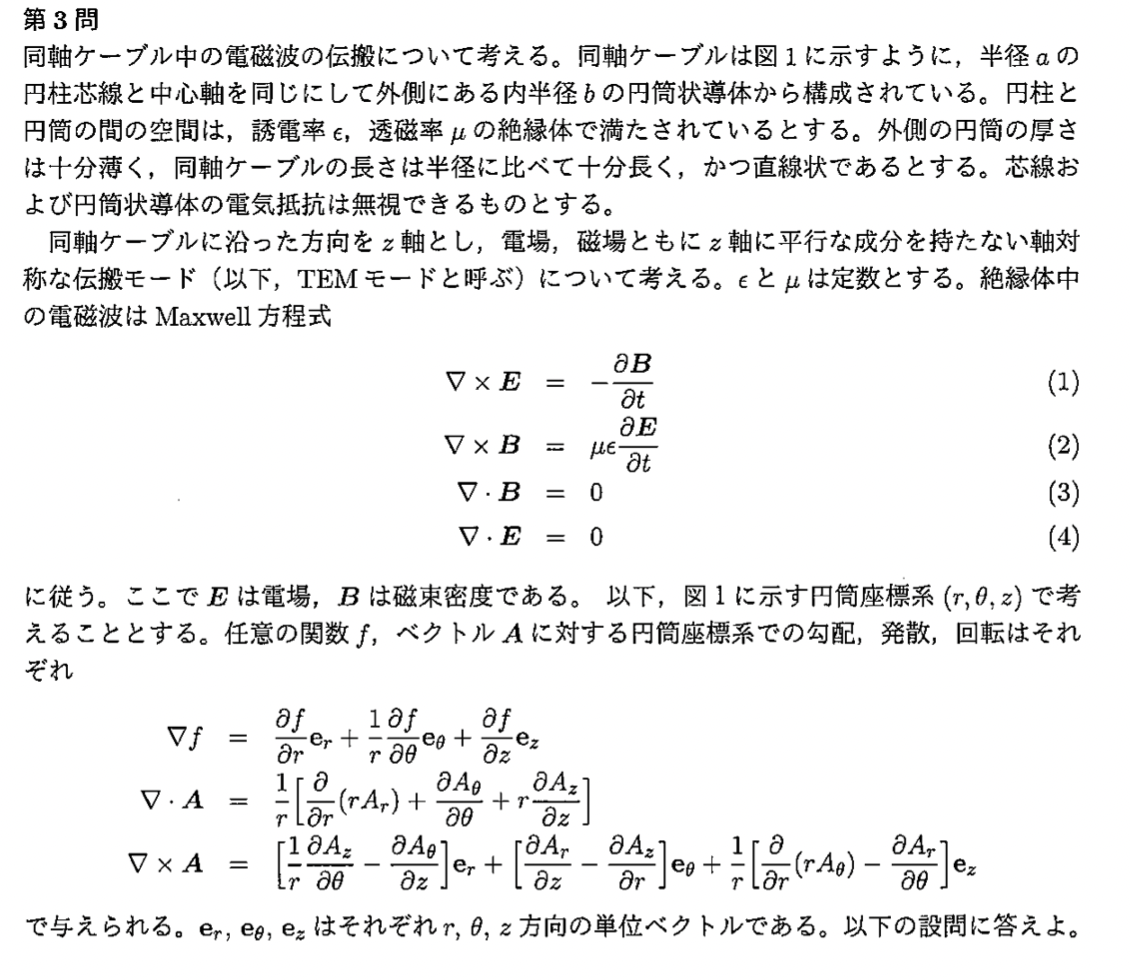
\includegraphics[width=0.7\linewidth,keepaspectratio]{./img/tokyoR4EM.png}
        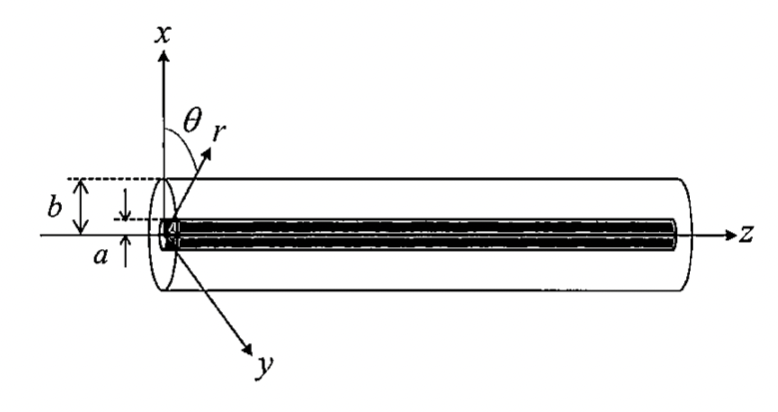
\includegraphics[width=0.7\linewidth,keepaspectratio]{./img/coaxial.png}
        % \caption{}
        \label{fig:}
    \end{figure}
    
    
    
    %\printbibliography[title='参考文献']
\end{document}